% Generated by plsimcount.pffigure -- do not edit; regenerate instead.
% figure: B-order4-by-formula -- Every order-4 formula at measured r
% source: results/pf-thesis/results.json
% metric=total gatebase=cz merged
% seed=1 t=n template=simcount synth=pygridsynth
% git_commit=04cd66abb614bdc66fb48e891cef085a299e0ab1 git_dirty=False
% source_sha256=018e0b7603e6fc9f6ee358974f241415a3b93437700847b033937cc1d4250db8
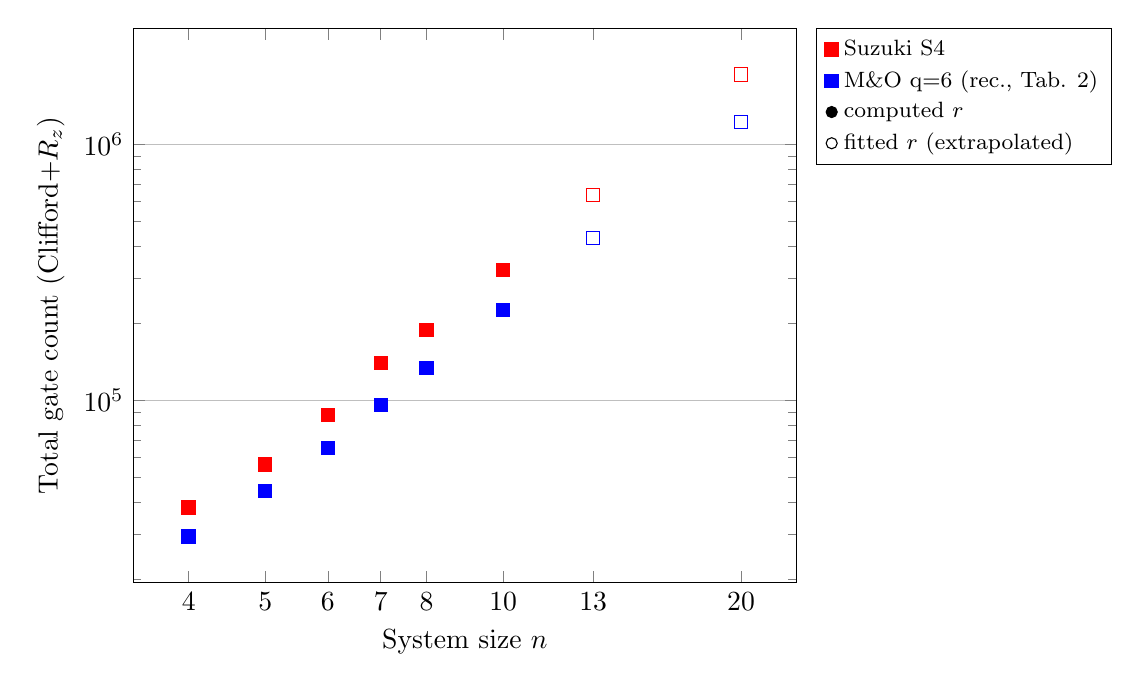
\begin{tikzpicture}
  \begin{loglogaxis}[
    width=10cm,
    xlabel={System size $n$},
    ylabel={Total gate count (Clifford+$R_z$)},
    xtick={4,5,6,7,8,10,13,20},
    xticklabels={4,5,6,7,8,10,13,20},
    ymajorgrids=true,
    legend pos=outer north east,
    legend cell align=left,
    legend style={font=\footnotesize},
  ]
    \addplot[only marks, red, mark=square*, mark size=2.4pt, mark options={solid, fill=red}] coordinates {
      (4,38160)
      (5,56180)
      (6,87768)
      (7,139496)
      (8,188256)
      (10,322240)
    };
    \addlegendentry{Suzuki S4}
    % r from power-law fit (extrapolation); one legend entry per series
    \addplot[only marks, red, mark=square*, mark size=2.4pt, mark options={solid, fill=white}, forget plot] coordinates {
      (13,633880)
      (20,1874080)
    };
    \addplot[only marks, blue, mark=square*, mark size=2.4pt, mark options={solid, fill=blue}] coordinates {
      (4,29348)
      (5,44275)
      (6,65274)
      (7,95634)
      (8,133584)
      (10,225170)
    };
    \addlegendentry{M\&O q=6 (rec., Tab. 2)}
    % r from power-law fit (extrapolation); one legend entry per series
    \addplot[only marks, blue, mark=square*, mark size=2.4pt, mark options={solid, fill=white}, forget plot] coordinates {
      (13,430859)
      (20,1219460)
    };
    \addlegendimage{only marks, black, mark=*, mark options={fill=black}}
    \addlegendentry{computed $r$}
    \addlegendimage{only marks, black, mark=*, mark options={fill=white}}
    \addlegendentry{fitted $r$ (extrapolated)}
  \end{loglogaxis}
\end{tikzpicture}
